\documentclass{standalone}
\usepackage{tikz}
\usetikzlibrary{patterns, positioning}

\begin{document}
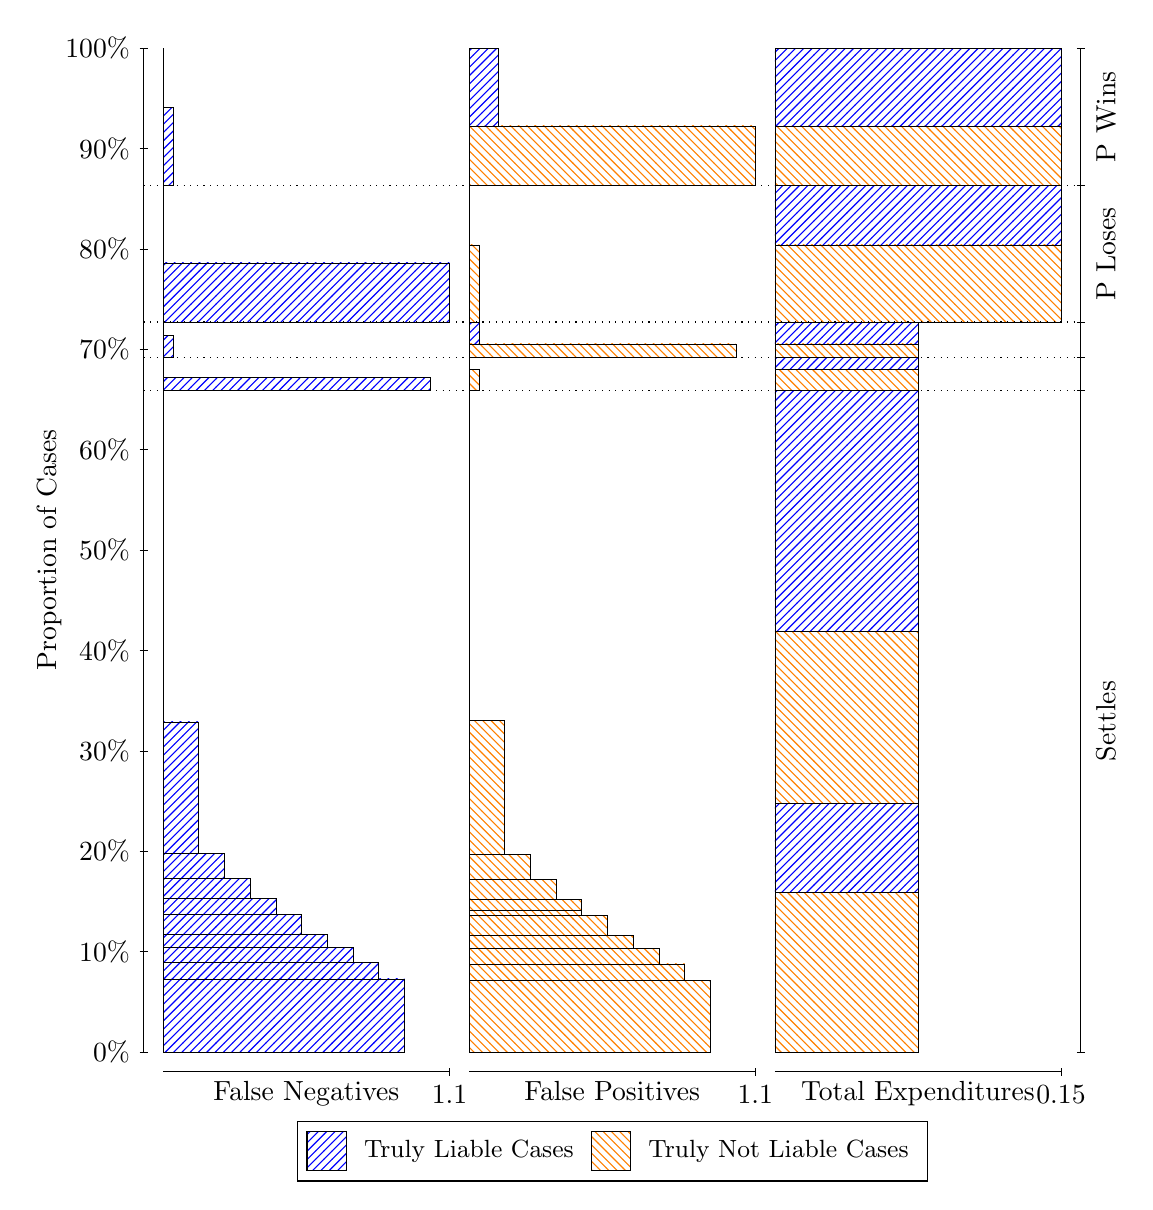
\begin{tikzpicture}
\draw[black, very thin] (1.5,1.75) -- (1.5,14.5);
\node[rotate=90, anchor=center] at (0.3, 8.125) {Proportion of Cases};
\draw[black, very thin] (1.45,1.75) -- (1.55,1.75);
\node[anchor=east] at (1.45, 1.75) {0\%};
\draw[black, very thin] (1.45,3.025) -- (1.55,3.025);
\node[anchor=east] at (1.45, 3.025) {10\%};
\draw[black, very thin] (1.45,4.3) -- (1.55,4.3);
\node[anchor=east] at (1.45, 4.3) {20\%};
\draw[black, very thin] (1.45,5.575) -- (1.55,5.575);
\node[anchor=east] at (1.45, 5.575) {30\%};
\draw[black, very thin] (1.45,6.85) -- (1.55,6.85);
\node[anchor=east] at (1.45, 6.85) {40\%};
\draw[black, very thin] (1.45,8.125) -- (1.55,8.125);
\node[anchor=east] at (1.45, 8.125) {50\%};
\draw[black, very thin] (1.45,9.4) -- (1.55,9.4);
\node[anchor=east] at (1.45, 9.4) {60\%};
\draw[black, very thin] (1.45,10.675) -- (1.55,10.675);
\node[anchor=east] at (1.45, 10.675) {70\%};
\draw[black, very thin] (1.45,11.95) -- (1.55,11.95);
\node[anchor=east] at (1.45, 11.95) {80\%};
\draw[black, very thin] (1.45,13.225) -- (1.55,13.225);
\node[anchor=east] at (1.45, 13.225) {90\%};
\draw[black, very thin] (1.45,14.5) -- (1.55,14.5);
\node[anchor=east] at (1.45, 14.5) {100\%};

\draw[black, very thin] (13.4,1.75) -- (13.4,14.5);
\draw[black, very thin] (13.35,1.75) -- (13.45,1.75);
\node[anchor=west] at (13.35, 1.75) {};
\draw[black, very thin] (13.35,10.154) -- (13.45,10.154);
\node[anchor=west] at (13.35, 10.154) {};
\draw[black, very thin] (13.35,10.575) -- (13.45,10.575);
\node[anchor=west] at (13.35, 10.575) {};
\draw[black, very thin] (13.35,11.02) -- (13.45,11.02);
\node[anchor=west] at (13.35, 11.02) {};
\draw[black, very thin] (13.35,12.753) -- (13.45,12.753);
\node[anchor=west] at (13.35, 12.753) {};
\draw[black, very thin] (13.35,14.5) -- (13.45,14.5);
\node[anchor=west] at (13.35, 14.5) {};

\draw[black, very thin, pattern color=blue, pattern=north east lines] (1.75,1.75) rectangle (4.8118,2.6776);
\draw[black, very thin, pattern color=blue, pattern=north east lines] (1.75,2.6776) rectangle (4.4852,2.8829);
\draw[black, very thin, pattern color=blue, pattern=north east lines] (1.75,2.8829) rectangle (4.1586,3.0773);
\draw[black, very thin, pattern color=blue, pattern=north east lines] (1.75,3.0773) rectangle (3.832,3.24);
\draw[black, very thin, pattern color=blue, pattern=north east lines] (1.75,3.24) rectangle (3.5054,3.4971);
\draw[black, very thin, pattern color=blue, pattern=north east lines] (1.75,3.4971) rectangle (3.1788,3.6973);
\draw[black, very thin, pattern color=blue, pattern=north east lines] (1.75,3.6973) rectangle (2.8522,3.9527);
\draw[black, very thin, pattern color=blue, pattern=north east lines] (1.75,3.9527) rectangle (2.5257,4.2731);
\draw[black, very thin, pattern color=blue, pattern=north east lines] (1.75,4.2731) rectangle (2.1991,5.9433);
\draw[black, very thin, pattern color=orange, pattern=north west lines] (1.75,5.9433) rectangle (1.75,10.154);
\draw[black, very thin, pattern color=blue, pattern=north east lines] (1.75,10.154) rectangle (5.1384,10.316);
\draw[black, very thin, pattern color=orange, pattern=north west lines] (1.75,10.316) rectangle (1.75,10.575);
\draw[black, very thin, pattern color=blue, pattern=north east lines] (1.75,10.575) rectangle (1.8725,10.853);
\draw[black, very thin, pattern color=orange, pattern=north west lines] (1.75,10.853) rectangle (1.75,11.02);
\draw[black, very thin, pattern color=blue, pattern=north east lines] (1.75,11.02) rectangle (5.3833,11.772);
\draw[black, very thin, pattern color=orange, pattern=north west lines] (1.75,11.772) rectangle (1.75,12.753);
\draw[black, very thin, pattern color=blue, pattern=north east lines] (1.75,12.753) rectangle (1.8725,13.743);
\draw[black, very thin, pattern color=orange, pattern=north west lines] (1.75,13.743) rectangle (1.75,14.5);
\draw[black, very thin, pattern color=orange, pattern=north west lines] (5.6333,1.75) rectangle (8.6951,2.6627);
\draw[black, very thin, pattern color=orange, pattern=north west lines] (5.6333,2.6627) rectangle (8.3685,2.8675);
\draw[black, very thin, pattern color=orange, pattern=north west lines] (5.6333,2.8675) rectangle (8.0419,3.0634);
\draw[black, very thin, pattern color=orange, pattern=north west lines] (5.6333,3.0634) rectangle (7.7154,3.2273);
\draw[black, very thin, pattern color=orange, pattern=north west lines] (5.6333,3.2273) rectangle (7.3888,3.4846);
\draw[black, very thin, pattern color=orange, pattern=north west lines] (5.6333,3.4846) rectangle (7.0622,3.5464);
\draw[black, very thin, pattern color=orange, pattern=north west lines] (5.6333,3.5464) rectangle (7.0622,3.6837);
\draw[black, very thin, pattern color=orange, pattern=north west lines] (5.6333,3.6837) rectangle (6.7356,3.937);
\draw[black, very thin, pattern color=orange, pattern=north west lines] (5.6333,3.937) rectangle (6.409,4.2598);
\draw[black, very thin, pattern color=orange, pattern=north west lines] (5.6333,4.2598) rectangle (6.0824,5.961);
\draw[black, very thin, pattern color=blue, pattern=north east lines] (5.6333,5.961) rectangle (5.6333,10.154);
\draw[black, very thin, pattern color=orange, pattern=north west lines] (5.6333,10.154) rectangle (5.7558,10.414);
\draw[black, very thin, pattern color=blue, pattern=north east lines] (5.6333,10.414) rectangle (5.6333,10.575);
\draw[black, very thin, pattern color=orange, pattern=north west lines] (5.6333,10.575) rectangle (9.0217,10.742);
\draw[black, very thin, pattern color=blue, pattern=north east lines] (5.6333,10.742) rectangle (5.7558,11.02);
\draw[black, very thin, pattern color=orange, pattern=north west lines] (5.6333,11.02) rectangle (5.7558,12.001);
\draw[black, very thin, pattern color=blue, pattern=north east lines] (5.6333,12.001) rectangle (5.6333,12.753);
\draw[black, very thin, pattern color=orange, pattern=north west lines] (5.6333,12.753) rectangle (9.2667,13.51);
\draw[black, very thin, pattern color=blue, pattern=north east lines] (5.6333,13.51) rectangle (6.0007,14.5);
\draw[black, very thin, pattern color=orange, pattern=north west lines] (9.5167,1.75) rectangle (11.333,3.7741);
\draw[black, very thin, pattern color=blue, pattern=north east lines] (9.5167,3.7741) rectangle (11.333,4.907);
\draw[black, very thin, pattern color=orange, pattern=north west lines] (9.5167,4.907) rectangle (11.333,7.094);
\draw[black, very thin, pattern color=blue, pattern=north east lines] (9.5167,7.094) rectangle (11.333,10.154);
\draw[black, very thin, pattern color=orange, pattern=north west lines] (9.5167,10.154) rectangle (11.333,10.414);
\draw[black, very thin, pattern color=blue, pattern=north east lines] (9.5167,10.414) rectangle (11.333,10.575);
\draw[black, very thin, pattern color=orange, pattern=north west lines] (9.5167,10.575) rectangle (11.333,10.742);
\draw[black, very thin, pattern color=blue, pattern=north east lines] (9.5167,10.742) rectangle (11.333,11.02);
\draw[black, very thin, pattern color=orange, pattern=north west lines] (9.5167,11.02) rectangle (13.15,12.001);
\draw[black, very thin, pattern color=blue, pattern=north east lines] (9.5167,12.001) rectangle (13.15,12.753);
\draw[black, very thin, pattern color=orange, pattern=north west lines] (9.5167,12.753) rectangle (13.15,13.51);
\draw[black, very thin, pattern color=blue, pattern=north east lines] (9.5167,13.51) rectangle (13.15,14.5);
\draw[black, dotted] (1.5,10.154) -- (13.4,10.154);
\draw[black, dotted] (1.5,10.575) -- (13.4,10.575);
\draw[black, dotted] (1.5,11.02) -- (13.4,11.02);
\draw[black, dotted] (1.5,12.753) -- (13.4,12.753);
\draw[black, very thin] (1.75,1.5) -- (5.3833,1.5);
\node[anchor=north] at (3.5667, 1.5) {False Negatives};
\draw[black, very thin] (5.3833,1.45) -- (5.3833,1.55);
\node[anchor=north] at (5.3833, 1.45) {1.1};

\draw[black, very thin] (5.6333,1.5) -- (9.2667,1.5);
\node[anchor=north] at (7.45, 1.5) {False Positives};
\draw[black, very thin] (9.2667,1.45) -- (9.2667,1.55);
\node[anchor=north] at (9.2667, 1.45) {1.1};

\draw[black, very thin] (9.5167,1.5) -- (13.15,1.5);
\node[anchor=north] at (11.333, 1.5) {Total Expenditures};
\draw[black, very thin] (13.15,1.45) -- (13.15,1.55);
\node[anchor=north] at (13.15, 1.45) {0.15};

\node[black, centered, rotate=90] at (13.72, 5.9522) {Settles};


\node[black, centered, rotate=90] at (13.72, 11.886) {P Loses};
\node[black, centered, rotate=90] at (13.72, 13.627) {P Wins};

\draw (7.449999999999999,1.5) node[draw=none] (baseCoordinate) {};
\begin{scope}[align=center]
        \matrix[scale=0.5, draw=black, below=0.5cm of baseCoordinate, nodes={draw}, column sep=0.1cm]{
            \node[rectangle, draw, minimum width=0.5cm, minimum height=0.5cm, pattern=north east lines, pattern color=blue] {}; &
            \node[draw=none, font=\small] (B) {Truly Liable Cases}; &
            \node[rectangle, draw, minimum width=0.5cm, minimum height=0.5cm, pattern=north west lines, pattern color=orange] {}; &
            \node[draw=none, font=\small] (B) {Truly Not Liable Cases}; \\
            };
\end{scope}

\end{tikzpicture}
\end{document}